\shorthandoff{:!} %règle un problème de compatibilité avec babel
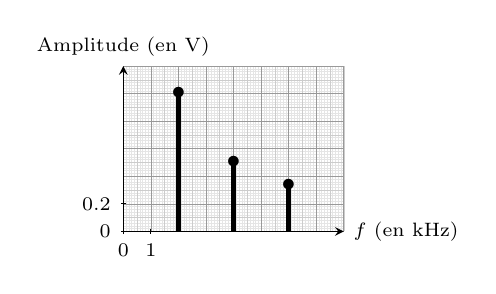
\begin{tikzpicture}[scale=0.35]
	
	%axes
		%papier milli
	\draw [very thin, gray!20] (0,0) grid[step=0.1] (8,6);
	\draw [very thin, black!20] (0,0) grid[step=0.5] (8,6);
	\draw [very thin, black!40] (0,0) grid[step=1] (8,6);
	%fin 
	%axes
	\draw[->,>=stealth] (0,0) -- (8,0) node[right] {\scriptsize{$f$ (en \si{kHz})}};
	%
	\draw[->,>=stealth] (0,-0.1) -- (0,6)node[above] {\scriptsize{Amplitude (en \si{V})}};
	\draw (0,0.1) -- (0,-0.1) node [below] {{\scriptsize $0$}}; %échelle abscisse
	\draw (1,0.1) -- (1,-0.1) node [below ] {{\scriptsize $1$}}; %échelle abscisse
	\draw (0.1,1) -- (-0.1,1) node [left] {{\scriptsize $\np{0.2}$}}; %échelle ordonnée
	\draw (0.1,0) -- (-0.1,0) node [left] {{\scriptsize $0$}}; %échelle ordonnée	% spectres 
	%%% raies 
	\draw [color=black,ultra thick, smooth, samples=250] (2,0) -- (2,5);
\draw (2,5) node {$\bullet$};
\draw [color=black,ultra thick, smooth, samples=250] (4,0) -- (4,2.5);
\draw (4,2.5) node {$\bullet$};
\draw [color=black,ultra thick, smooth, samples=250] (6,0) -- (6,1.66);
\draw (6,1.66) node {$\bullet$};
\end{tikzpicture} 
\shorthandon{:!}